\chapter{Scepia}\thumbforchapter
\chapterauthor{Rebecca Snabel*, Maarten van der Sande*, Gert Jan Veenstra, Simon J. van Heeringen}
\newpage

\section{Introduction}

\section{Methods}

\subsection{Data collection}

This is from ANANSE:
To generate a collection of putative enhancer regions, we collected all transcription factor ChIP-seq peaks from ReMap 2018 (\href{http://remap.univ-amu.fr/storage/remap2018/hg38/MACS/remap2018_all_macs2_hg38_v1_2.bed.gz}{http://remap.univ-amu.fr/storage/remap2018/hg38/MACS/remap2018\_all\_macs2\_hg38\_v1\_2.bed.gz}) (\href{javascript:;}{41}). We took the summit of all peaks and extended these 25 bp up- and downstream. Based on this file, we generated a coverage bedGraph using bedtools genomecov (\href{javascript:;}{78}). We performed peak calling on this bedGraph file using bdgpeakcall from MACS2 (version v2.7.1) (\href{javascript:;}{69}), with the following settings: \textit{l} = 50 and \textit{g} = 10. We performed the peak calling twice, setting \textit{c} to 4 and 30, respectively. All peaks from \textit{c} = 30 were combined with all peaks of \textit{c} = 4 that did not overlap with the peaks of \textit{c} = 30. We then removed all regions on chrM and extended the summit of the peaks 100 bp up- and downstream to generate a final collection of 1 268 775 putative enhancers of 200 bp. This collection of enhancers is available at Zenodo with doi 10.5281/zenodo.4066423.

Regulatory potential database was made by downloading all human bam files from ENCODE and mapping against REMAP.

Preprocessing of RNA-seq was done automatically by seq2science v1.0.3 \cite{seq2science} using the rna-seq workflow. Public samples were downloaded from the Sequence Read Archive \cite{Leinonen2010} with help of the ncbi e-utilities and pysradb\cite{Choudhary2019}. Genome assembly GRCh38.p13 was downloaded with genomepy 0.16.1 \cite{Frlich2023}. Paired-end reads were trimmed with fastp v0.23.2 \cite{Chen2018} with default options. Reads were aligned with STAR v2.7.10b \cite{Dobin2012} with default options. Afterwards, duplicate reads were marked with Picard MarkDuplicates v3.0.0 \cite{picard}. Bam files were converted to cram format with samtools samtools v1.16 \cite{Danecek2021}. Read counting and summarizing to gene-level was performed on filtered bam using HTSeq-count v2.0.2 \cite{Anders2014}. TPM normalized gene counts were generated using genomepy based on longest transcript lengths.

\subsection{Bulk comparison}

 

\subsection{Single-cell comparison}


\subsection{Scepia}

\begin{figure}
    \centering
    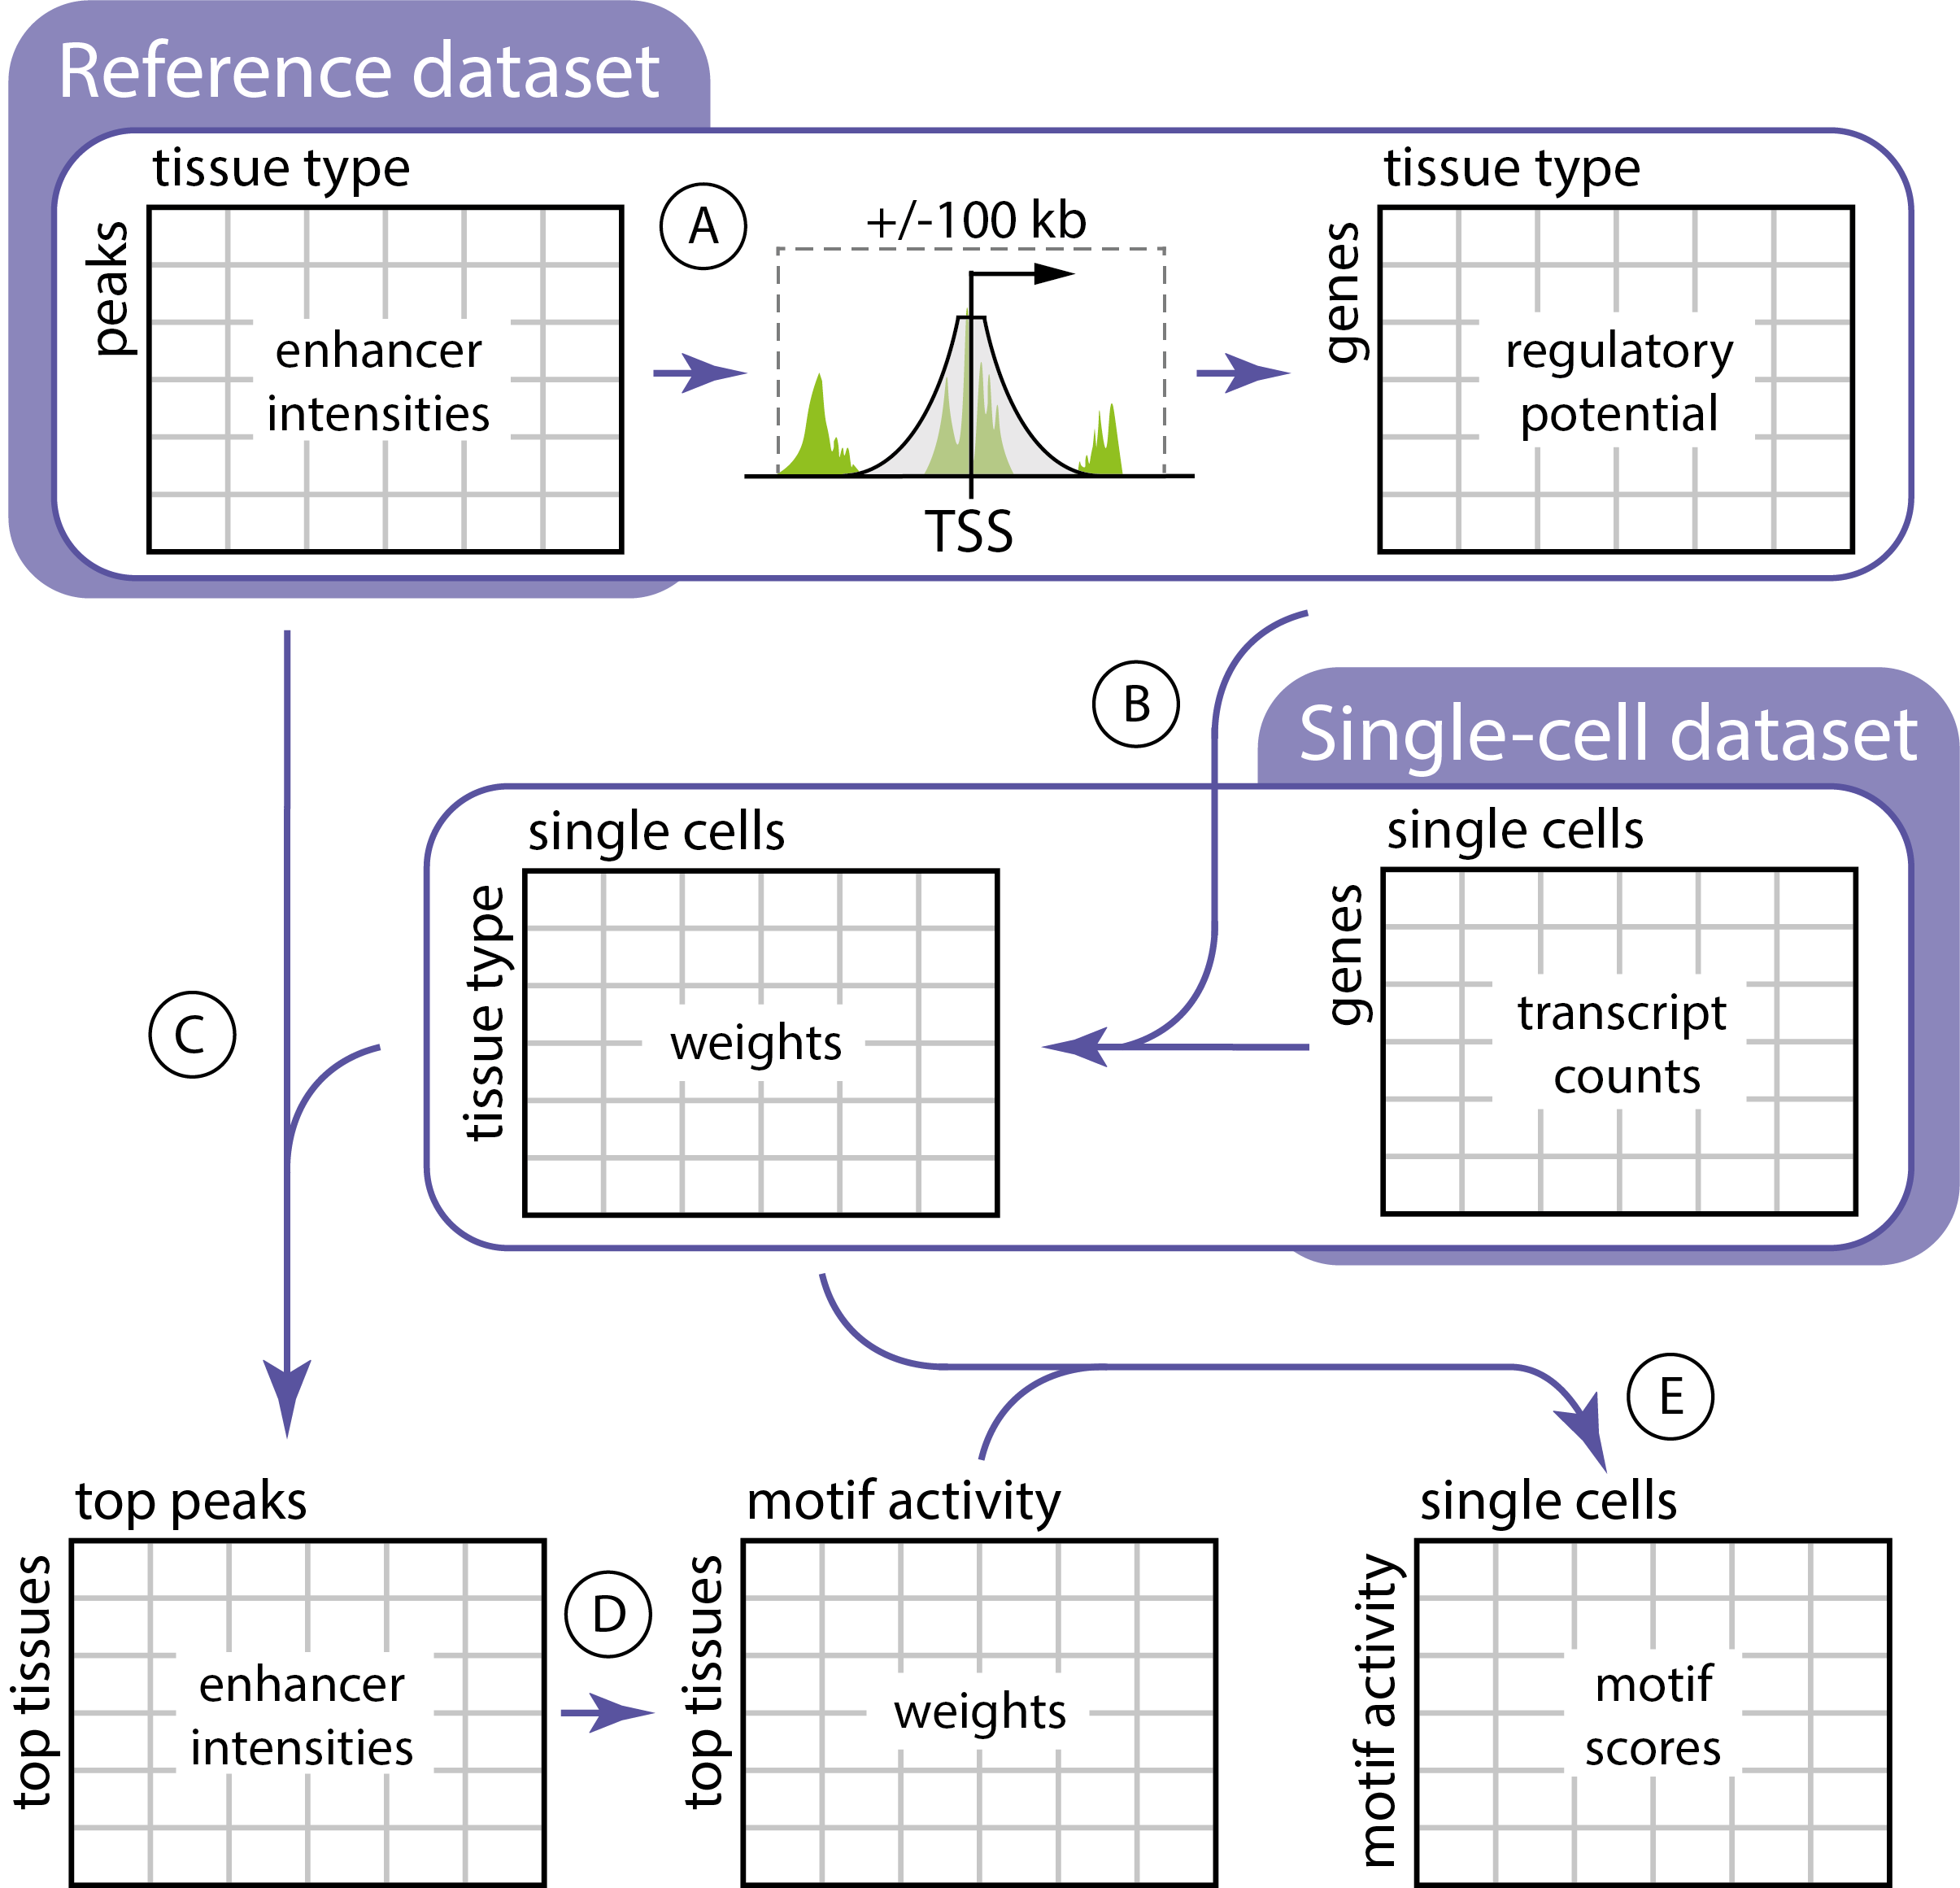
\includegraphics[width=1\linewidth]{ch.scepia/imgs/overview.png}
    \caption{TODO caption}
    \label{fig:enter-label}
\end{figure}

\noindent
Input:

\begin{itemize}
	\item Reference database matrix of peak intensities (D) with dimensions (peaks x cell types). Scepia comes with multiple extensive reference databases, and user does not need to provide themselves.
    \begin{itemize}
    \item The peaks are REMAP
    \item The different cell types from ENCODE.
    \item The values are the quantile normalized log1p (IS THIS TRUE?) counts.
    \item H3K27ac, but can also be ATAC seq or ...
    \end{itemize}
	\item Single-cell RNA-seq dataset S with dimensions (cells x genes). 
    \begin{itemize}
        \item ...?
    \end{itemize}
\end{itemize}

% TODO TISSUE TYPES OR CELL TYPES? Or sth else?

\noindent
This is how scepia works:

\begin{enumerate}
    \item Convert the reference database matrix of peak intensities D into a database matrix of regulatory potential per gene (P) with dimensions (genes x cell types). The reference database includes all REMAP peaks, so including promoters, and is made beforehand. 
    \begin{itemize}
        \item The regulatory potential of gene $g$ is calculated as: \begin{equation*}{P_{g}} = \sum\limits_k {{w_{k}}{s_{k,g}}\ } \end{equation*}
where $w_k$ is the weight at position $k$ and $s_{k,g}$ the h3k27ac signal at position $k$ for gene $g$.
        \item The weight function is calculated similar to ANANSE: \begin{equation*} w_k=\left\{\begin{matrix} 1, && k\epsilon (0\,{\rm kb},\ 5\,{\rm kb}]\\ \frac{2{\rm e}^{-\mu|k-t_g|} }{1+{\rm e}^{-\mu|k-t_g|}}, && k\epsilon (5\,{\rm kb},\ 100\,{\rm kb}] \end{matrix}\right. \end{equation*}
where parameter $t_g$ is the genomic position of the TSS of gene $g$, and $\mu$ determines the decay rate as a function of distance from the TSS, is set such that an enhancer 10 kb from the TSS contributes one-half of an enhancer within 5 kb from TSS. $t_g$ is the distance
    \end{itemize}

    \item Weigh each cell in the single-cell dataset (S) with regulatory potential (P) resulting in annotation matrix A with dimensions (cells x cell types).
    \begin{itemize}
        \item We do a lasso regression to infer the annotation weights: $S_i = P_i A_i + \lambda ||A_i||_1 +\epsilon$
        \item this is much more complex, as we first take cluster most common, then do it for each cell based on average neighbour gene expression, and finally, take the average cell type annotation of the neighbours..
    \end{itemize}

    \item Keep the most important cell / tissue types, and look up the top differential \textit{enhancers} between these tissue types.

    \item Do a (differential) motif scan over the differential enhancers. 
    \begin{itemize}
        \item We do a bayesian ridge regression to infer the motif weights TODO formula: $S_i = P_i A_i + \lambda ||A_i||_2^2 +\epsilon$
        \item TODO ridge is $ \underset{\beta}{\operatorname{arg\,min}}\; \|y - X\beta\|^2_2 + \lambda \|\beta\|^2_2 $
    \end{itemize}
    
    \item dot product of annotation weights and motif scores F
    \begin{itemize}
        \item $F = S \cdot A$
    \end{itemize}

    \item THIS NEEDS TO BE ADDED. Correlate motif scores and transcript scores between cells. This is used to determine significance.
    

\end{enumerate}

\section{Results}

\subsection{Matching regulatory potential and RNA}

To examine the relationship between regulatory potential and RNA-seq, we downloaded X human RNA-seq cell types and Y human H3K27ac cell types from ENCODE. We then calculated the correlation coefficient between all permutations of regulatory potential and RNA-seq TPM (Fig. \ref{fig:celltypes}). The average correlation coefficient between the same cell types is $0.53 \pm 0.14$, and in $64\%$ of the cases the regulatory potential of a tissue had the highest correlation coefficicient with the TPM of the same tissue type. Broadening XXX resulted in a $77\%$ correct annotation. The exact parameters for the calculation of the regulatory potential does not particularly matter, as the signal in the promoter is enough to predict TPM. As such we think that the H3K27ac regulatory potential signal is a good (decent?) classifier for cell state.

The relationship between RNA-seq and regulatory potential led us to the question of whether a reference database of H3K27ac signal and 

\begin{figure}
    \centering
    \includegraphics[width=0.75\linewidth]{ch.scepia/imgs/celltypes.png}
    \caption{Ill encircle some stuff for convincing. Not sure which cmap, all are ugly.. or not colorblind, or red green and thats confusing microarray. Also Ill remove labels in the end?}
    \label{fig:celltypes}
\end{figure}
Since a gene's transcript counts and its regulatory potential are correlated, 
\begin{figure}
    \centering
    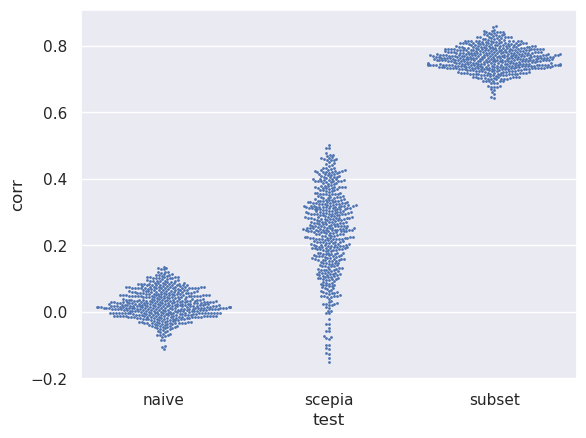
\includegraphics[width=0.75\linewidth]{ch.scepia/imgs/scepia_bulk_benchmark.png}
    \caption{}
    \label{fig:enter-label}
\end{figure}
See supplemental figure XXX for parameter sweep. This is nice because test/validate separate

\subsection{Single-Cell Epigenome-based Inference of Activity}

\section{Discussion}

\subsection{Limitations}
\begin{itemize}
    \item Benchmark is bad. Benchmarking against a bad ground truth is stupid.
    \item 
\end{itemize}

\section{Supplementals}
\beginsupplement
\begin{table}
\begin{center}
\begin{tabular}{||c c c c||} 
\hline
Weight curve & Correlation between & Correct specific & Correct broad \\[0.5ex] 
\hline
Ananse & $0.53 \pm 0.14$ & $64\%$ & $77\%$ \\ 
\hline
Wang & $0.54 \pm 0.15 $ & $64\%$ & $75\%$ \\
\hline
Promoter (5kb) & $0.54 \pm 0.14$ & $66\%$ & $77\%$ \\
\hline
Enhancer & $0.43 \pm 0.14$ & $60\%$ & $72\%$ \\
\hline
\end{tabular}
\caption{Caption of my table.}
\label{table:1}
\end{center}
\end{table}
